\documentclass[a4paper,12pt]{article}
%For links
%\usepackage{url}
%For images
\usepackage{graphicx}
 
\addtolength{\oddsidemargin}{-.875in}
\addtolength{\evensidemargin}{-.875in}
\addtolength{\textwidth}{1.75in}
 
\addtolength{\topmargin}{-.875in}
\addtolength{\textheight}{1.75in}
 
\begin{document}
\begin{enumerate}
      \item $$sin(2x)=0.875$$
            Med en miniräknare tar man $sin^{-1}$ på båda sidorna och räknar ut
            $$2x+2\pi n=sin^{-1}(0.875)+2\pi n \Rightarrow x=\frac{sin^{-1}(0.875)+2\pi n}{2}\approx 0.533+\pi n$$

            Rent geometriskt kan det beskrivas nedan.

            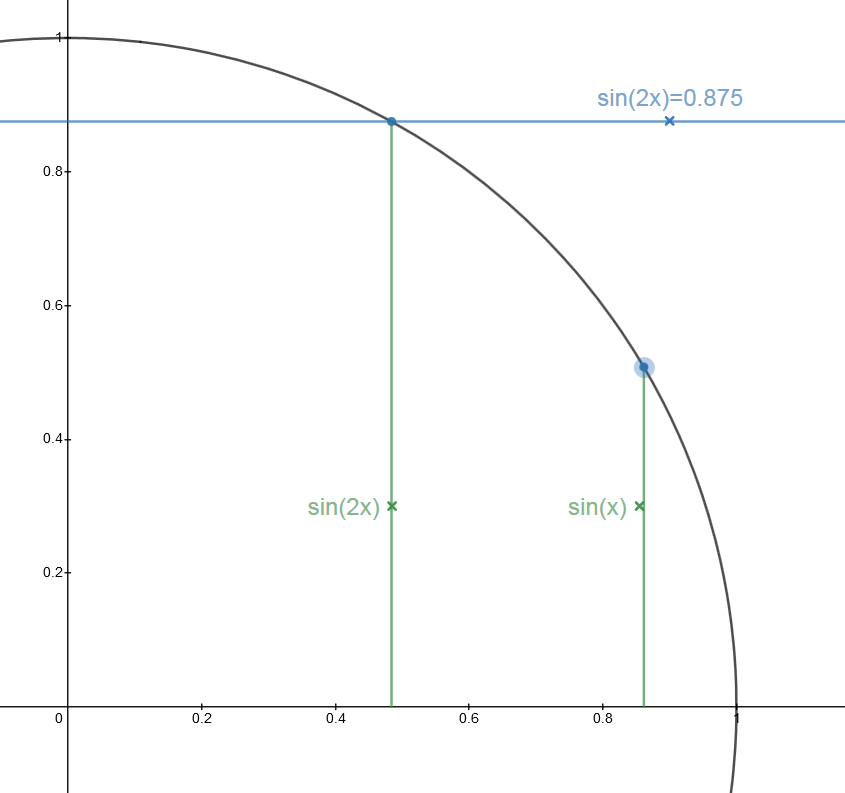
\includegraphics[scale=0.5]{Figur1.png}

            Det andra svaret är sker då på andra sidan cirkeln
            $$2x+2\pi n=\pi - sin^{-1}(0.875)+2\pi n \Rightarrow x=\frac{\pi - sin^{-1}(0.875)+2\pi n}{2}\approx 1,304+\pi n$$

      \item \begin{enumerate}
                  \item Följande ekvation konverterar från radier till grader $2.5\cdot180^\circ/\pi\approx 140$ grader.

                  \item Man konverterar grader till radier med $36^\circ\pi/180^\circ\approx 0.63$ radier.
            \end{enumerate}
      \item
            \begin{enumerate}
                  \item Man kan rita $y=cos(2x)$ genom att tänka sig en pendel som åker igenom cirkeln dubbelt
                        så snabbt som den vanliga pendeln. Då kommer varje vinkel x nås dubbelt så snabbt. Då blir
                        cos(2x) för 45 graders vinkeln $\pi/4=0$. Vid $\pi/2$ är det då -1 osv.

                        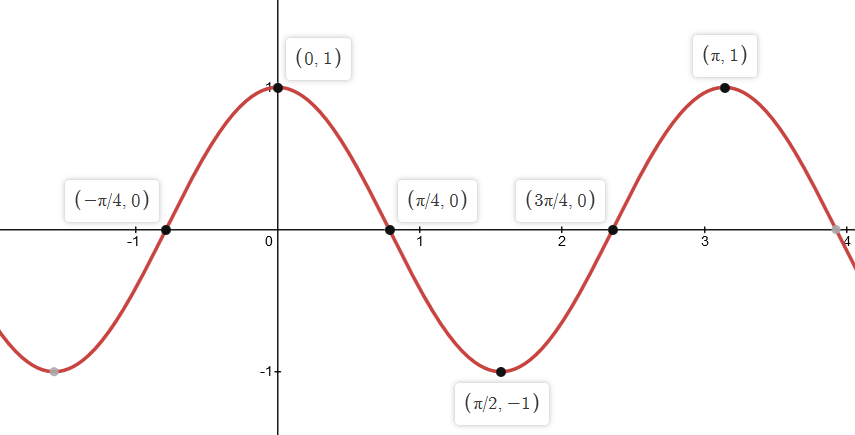
\includegraphics[scale=0.7]{Figur2.png}

                  \item Det första man kan ta reda på är noll punkterna. Det sker vid $\pi/6$ och $7\pi/6$,
                        eller generellt vid $(1+6n)\pi/6$.
                        Detta är för att $pi/6$ i ekvationen är fasen som skiftar vart pendeln börjar.
                        Maxpunktens x-position kommer ligga vid genomsnittet
                        av nollpunkterna dvs $\frac{\pi/6+7\pi/6}{2}=\frac{8\pi}{12}=\frac{2\pi}{3}$, och eftersom
                        amplituden är 3 så kommer y-positionen vara 3. Då får vi grafen

                        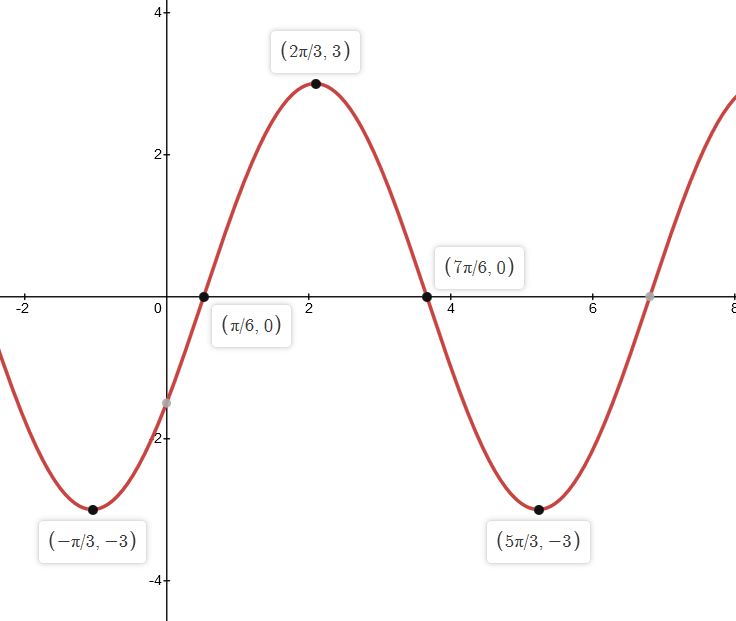
\includegraphics[scale=0.5]{Figur3.png}
            \end{enumerate}

      \item Börja med att dela båda sidorna med sin(x)
            $$2cos(x)=1$$
            $$cos(x)=1/2$$
            Detta sker när $x=60^\circ$ så svaret är $60^\circ + 360n, n \in \mathbf{Z}$.

      \item \begin{enumerate}
                  \item cos(t) är som störst vid $t=0$ och $t=\pi$. t=0 blir enklare
                        att räkna ut, så
                        $$3+1.5cos(0.1\pi \cdot 0)=4.5$$
                        Så då blir maxdjupet 4.5 meter. Detta stämmer även överens grafiskt.
                  \item Frågan kan ställas om till "när är ekvationen lika med 4?"
                        $$3+1.5cos(\pi t/10)=4$$
                        Och kan då lösas som följande
                        $$cos(\pi t/10)=2/3$$
                        $$t=10cos^{-1}(2/3)/\pi \approx 2.677$$
                        Detta kan man verifiera grafiskt:

                        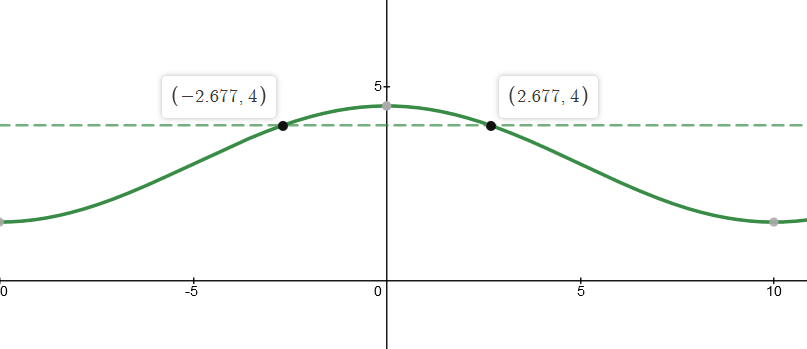
\includegraphics[scale=0.55]{Figur4.png}

            \end{enumerate}

      \item Detta kan lösas genom att finna skärningspunkterna mellan
            funktionerna $sin^2(x)-1$ och $1.5sin(x)$ som visas nedan.

            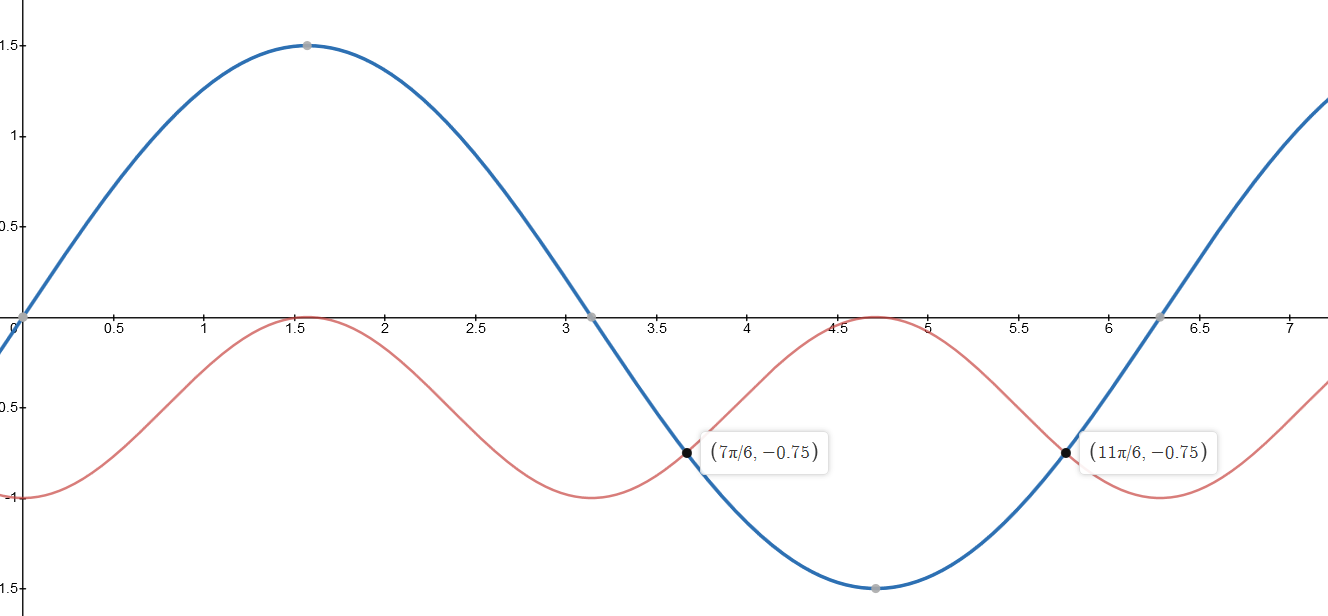
\includegraphics[scale=0.45]{Figur5.png}

            Svaren blir då $7\pi/6 +2\pi n$ och $11\pi/6 +2\pi n$

      \item Grafiskt ser det ut som följande
            där man även kan observera grafens skärningspunkter

            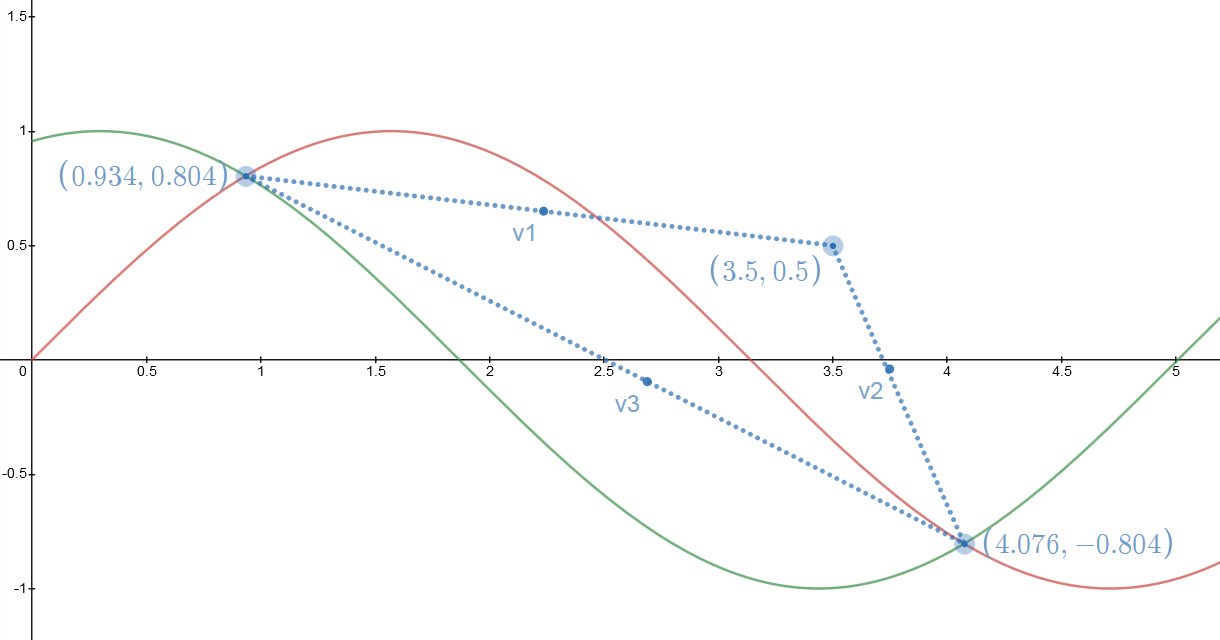
\includegraphics[scale=0.5]{Figur6.png}

            Då kan varenda linje i triangeln bli sin egna vektor $\vec{v_i}=(x,y)^T$, där
            x är den högra punktens x-koordinat minus den vänstra punktens x, och där y är den högra punktens y minus
            den vänstra punkten y (inte den övre eller undre).
            Den euklidiska längden $||v_1||$ är då pythagoras sats som räknas ut nedan.

            $$||v_1||=\sqrt{(3.5-0.934)^2+(0.5-0.804)^2}=2.584$$
            $$||v_2||=\sqrt{(3.5-4.076)^2+(0.5-(-0.804))^2}=1.426$$
            $$||v_3||=\sqrt{(0.934-4.076)^2+(0.804-(-0.804))^2}=3.529$$

            Triangelns omkrets blir då summan av vektorernas längder
            $$||v_1||+||v_2||+||v_3||=2.584+1.426+3.529=7.539$$
            Som då är svaret på frågan.
\end{enumerate}
\end{document}

